\documentclass{article}

\title{Introduction to GeoDaSpace: A Desktop Program for Spatial Regression and Diagnostics}
\author{Luc Anselin, Pedro Amaral, Daniel Arribas-Bel and David Folch}
%\date{}

\usepackage{amsmath}
\usepackage{natbib}
\bibpunct{(}{)}{,}{a}{}{,}
\usepackage{float}
\usepackage{xcolor}
\usepackage{amssymb} 
\usepackage{listings}
\usepackage{caption}
\usepackage{hyperref}
\usepackage{subfig}
\usepackage{color,soul}
\usepackage[section]{placeins}
\usepackage{graphicx}
\graphicspath{{figures/}}
\DeclareCaptionFont{white}{\color{white}}
\DeclareCaptionFormat{listing}{%
  \parbox{\textwidth}{\colorbox{gray}{\parbox{\textwidth}{#1#2#3}}\vskip-4pt}}
\captionsetup[lstlisting]{format=listing,labelfont=white,textfont=white}
\lstset{frame=lrb,xleftmargin=\fboxsep,xrightmargin=-\fboxsep}
\newfloat{code}{H}{myc}

\begin{document}

\maketitle
\thispagestyle{empty}

\vfill

\begin{figure}[htb]
\begin{center}

\includegraphics[width=0.5\linewidth]{geodaspace.png}\\
\end{center}
\end{figure}

\vfill

\begin{figure}[htb]
\begin{center}

\includegraphics[width=0.75\linewidth]{GeodaLogo.png}\\
\end{center}
\end{figure}


\clearpage
\pagestyle{plain}

\setcounter{secnumdepth}{3} 
\setcounter{tocdepth}{2}   

\renewcommand\contentsname{Table of Contents}
\tableofcontents

\newpage
%\listoffigures	
%\newpage
%\listoftables 



\section{Introduction}
\label{s:intro}

This document provides a first introduction to the use of GeoDaSpace (Section \ref{s:GS}) and compares estimation results using GeoDaSpace, Stata and R (Section \ref{s:comparisons}). In instances where results differ between the three programs, we document why this is the case.

GeoDaSpace is a free desktop program to obtain results from spatial diagnostic tests and to estimate spatial regression parameters.\footnote{The alpha version of the program can be downloaded at https://geodacenter.asu.edu/software/downloads/geodaspace.} It is developed by Dr. Luc Anselin and his team at the GeoDa Center for Geospatial Analysis and Computation, which is part of the School of Geogaphical Sciences and Urban Planning at Arizona State University.\footnote{The team contributions of Dr. Daniel Arribas-Bel, Pedro V. Amaral, Dr. David Folch, Nick Malizia, Charles Schmidt, Ran Wei, Jing Yao, Phil Stephens, Dr. Mark McCann, and Dr. Julia Koschinsky are gratefully acknowledged. We also appreciate the valuable feedback from analysts who tested the alpha versions of GeoDaSpace. For information about the GeoDa Center, see  \url{https://geodacenter.asu.edu}} The software provides a graphical user interface (GUI) for the spatial regression module \emph{spreg} that was initially released as part of PySAL 1.3 on July 31, 2012 \citep{Rey07}. PySAL is an open source library for spatial analysis written in the programming language Python.\footnote{More information about PySAL can be found at \url{http://pysal.org/}}  The project is directed by Dr. Serge Rey at the GeoDa Center.

The main methods and models implemented in GeoDaSpace are listed in Table \ref{t:methods}. They include Ordinary Least Squares (OLS), Two-Stage Least Squares (TSLS), and General Methods of Moments (GMM) to estimate the spatial lag model, the spatial error model, and the spatial lag + error model.  The estimation of the spatial lag model is based on spatial two-stage least squares (STSLS) \citep{Anselin88}. For the estimation of the spatial error and lag and error models the methods developed by \citet{Kelejian98,Kelejian99} (KP98/99) and \citet{Drukker10} (KPD) are implemented, in addition to the heteroskedasticity robust method proposed by \citet{Arraiz10} (KP-Het).  

Spatial and non-spatial diagnostics can be obtained for all of these estimation methods in GeoDaSpace. Further, non-spatial endogenous variables can be specified and heteroskedasticity corrections are available (heteroskedasticity and autocorrelation consistent (HAC) \citep{Kelejian07} and White's heteroskedasticity consistent covariance matrix \citep{White80}). GeoDaSpace also offers utilities to create and manipulate weights matrices based on contiguity, distance (bands, KNN, inverse distance) and kernels.

Table \ref{t:methods} also shows the methods provided in GeoDaSpace that can be found in Stata and R. For this document we consider two different versions of the R package \emph{sphet} developed by Dr. Gianfranco Piras. The first one, \emph{sphet1}, is the released version of \emph{sphet} (v. 1.1-12, published on CRAN on 2012-04-13). In addition, we use the alpha version from R-Forge, revision 56, published on 2012-07-22. This newer version of the code, which contains additional methods and enhancements to \emph{sphet1}, is subsequently referred to as \emph{sphet2}.\footnote{Please note that, as an alpha version, this code is subject to change.}


\begin{table}[htpb]
\caption{Methods and models implemented in GeoDaSpace and their availability in Stata and R}
\label{t:methods}
\centering
\begin{small}
\begin{tabular}{l|cccc} \hline
\textbf{Method}&\textbf{GeoDaSpace}&\textbf{Stata}&\textbf{R$^1$}&\textbf{R$^2$}\\ \hline
Standard (OLS) &{\LARGE$\textcolor{blue}\bullet$}&{\LARGE$\textcolor{blue}\bullet$}&{\LARGE$\textcolor{blue}\bullet$}&{\LARGE$\textcolor{blue}\bullet$}\\
\textcolor{white}{XXX} with heteroskedasticity (White)&{\LARGE$\textcolor{blue}\bullet$}&{\LARGE$\textcolor{blue}\bullet$}&{\LARGE$\textcolor{blue}\bullet$}&{\LARGE$\textcolor{blue}\bullet$}\\
\textcolor{white}{XXX} with heteroskedasticity (HAC)&{\LARGE$\textcolor{blue}\bullet$}&&{\LARGE$\textcolor{blue}\bullet$}&{\LARGE$\textcolor{blue}\bullet$}\\
Standard (TSLS)&{\LARGE$\textcolor{blue}\bullet$}&{\LARGE$\textcolor{blue}\bullet$}&{\LARGE$\textcolor{blue}\bullet$}&{\LARGE$\textcolor{blue}\bullet$}\\
\textcolor{white}{XXX} with endogenous var and het. (White)&{\LARGE$\textcolor{blue}\bullet$}&{\LARGE$\textcolor{blue}\bullet$}&{\LARGE$\textcolor{blue}\bullet$}&{\LARGE$\textcolor{blue}\bullet$}\\
\textcolor{white}{XXX} with endogenous var. and het. (HAC)&{\LARGE$\textcolor{blue}\bullet$}&&{\LARGE$\textcolor{blue}\bullet$}&{\LARGE$\textcolor{blue}\bullet$}\\
Spatial lag (STSLS)&{\LARGE$\textcolor{blue}\bullet$}&{\LARGE$\textcolor{blue}\bullet$}&{\LARGE$\textcolor{blue}\bullet$}&{\LARGE$\textcolor{blue}\bullet$}\\
\textcolor{white}{XXX} with het. (White)&{\LARGE$\textcolor{blue}\bullet$}&{\LARGE$\textcolor{blue}\bullet$}&{\LARGE$\textcolor{blue}\bullet$}&{\LARGE$\textcolor{blue}\bullet$}\\
\textcolor{white}{XXX} with het. (HAC)&{\LARGE$\textcolor{blue}\bullet$}&&{\LARGE$\textcolor{blue}\bullet$}&{\LARGE$\textcolor{blue}\bullet$}\\
\textcolor{white}{XXX} with endogenous var.&{\LARGE$\textcolor{blue}\bullet$}&{\LARGE$\textcolor{blue}\bullet$}&&{\LARGE$\textcolor{blue}\bullet$}\\
\textcolor{white}{XXX} with endog. var. and het. (White)&{\LARGE$\textcolor{blue}\bullet$}&{\LARGE$\textcolor{blue}\bullet$}&&{\LARGE$\textcolor{blue}\bullet$}\\
\textcolor{white}{XXX} with endog. var. and het. (HAC) &{\LARGE$\textcolor{blue}\bullet$}&&&{\LARGE$\textcolor{blue}\bullet$}\\
Spatial error (GM) (KP98/99)&{\LARGE$\textcolor{blue}\bullet$}&{\LARGE$\textcolor{blue}\bullet$}&{\LARGE$\textcolor{blue}\bullet$}&{\LARGE$\textcolor{blue}\bullet$}\\
\textcolor{white}{XXX} with endogenous var. &{\LARGE$\textcolor{blue}\bullet$}&{\LARGE$\textcolor{blue}\bullet$}&&\\
Spatial error and lag (GM) (KP98/99)&{\LARGE$\textcolor{blue}\bullet$}&{\LARGE$\textcolor{blue}\bullet$}&{\LARGE$\textcolor{blue}\bullet$}&{\LARGE$\textcolor{blue}\bullet$}\\
\textcolor{white} {XXX} with endog. var. &{\LARGE$\textcolor{blue}\bullet$}&{\LARGE$\textcolor{blue}\bullet$}&&\\
Spatial error (GMM)(KPD)&{\LARGE$\textcolor{blue}\bullet$}&{\LARGE$\textcolor{blue}\bullet$}&&{\LARGE$\textcolor{blue}\bullet$}\\
\textcolor{white}{XXX} with endogenous var. &{\LARGE$\textcolor{blue}\bullet$}&{\LARGE$\textcolor{blue}\bullet$}&&{\LARGE$\textcolor{blue}\bullet$}\\
Spatial error and lag (GMM) (KPD)&{\LARGE$\textcolor{blue}\bullet$}&{\LARGE$\textcolor{blue}\bullet$}&&{\LARGE$\textcolor{blue}\bullet$}\\
\textcolor{white}{XXX} with endog. var. &{\LARGE$\textcolor{blue}\bullet$}&{\LARGE$\textcolor{blue}\bullet$}&&{\LARGE$\textcolor{blue}\bullet$}\\
Spatial error with heteroskedasticity (GMM) (KP-Het)&{\LARGE$\textcolor{blue}\bullet$}&{\LARGE$\textcolor{blue}\bullet$}&{\LARGE$\textcolor{blue}\bullet$}&{\LARGE$\textcolor{blue}\bullet$}\\
\textcolor{white}{XXX} with endog. var. and het. &{\LARGE$\textcolor{blue}\bullet$}&{\LARGE$\textcolor{blue}\bullet$}&&{\LARGE$\textcolor{blue}\bullet$}\\
Spatial error and lag with het. (GMM) (KP-Het)&{\LARGE$\textcolor{blue}\bullet$}&{\LARGE$\textcolor{blue}\bullet$}&{\LARGE$\textcolor{blue}\bullet$}&{\LARGE$\textcolor{blue}\bullet$}\\
\textcolor{white}{XXX} with endog. var. and het. &{\LARGE$\textcolor{blue}\bullet$}&{\LARGE$\textcolor{blue}\bullet$}&&{\LARGE$\textcolor{blue}\bullet$}\\
\hline
\multicolumn{5}{l}{\scriptsize{$^1$R packages spdep and sphet (v. 1.1-12, published on CRAN on 2012-04-13).}} \\
\multicolumn{5}{l}{\scriptsize{$^2$R packages spdep and sphet (revision 56, published on R-Forge on 2012-07-22).}} \\
\end{tabular}
\end{small}
\end{table}


\newpage
\section{Using GeoDaSpace}
\label{s:GS}
\subsection{Opening a Data File and Specifying a Model}

GeoDaSpace is a stand-alone software program that provides a graphical user interface (GUI) for PySAL's spatial regression module  \emph{spreg}. It is available for the Windows and Mac OSx platforms and can be downloaded for free from the GeoDaCenter's software page: \url{https://geodacenter.asu.edu/software}. 

The main GUI window is shown in Figure \ref{f:gui}. It contains four main sections: The menu icons (top), data and weights utilities (left), model specification (right) and model estimation (bottom). 

\begin{figure}[htb]
\begin{center}
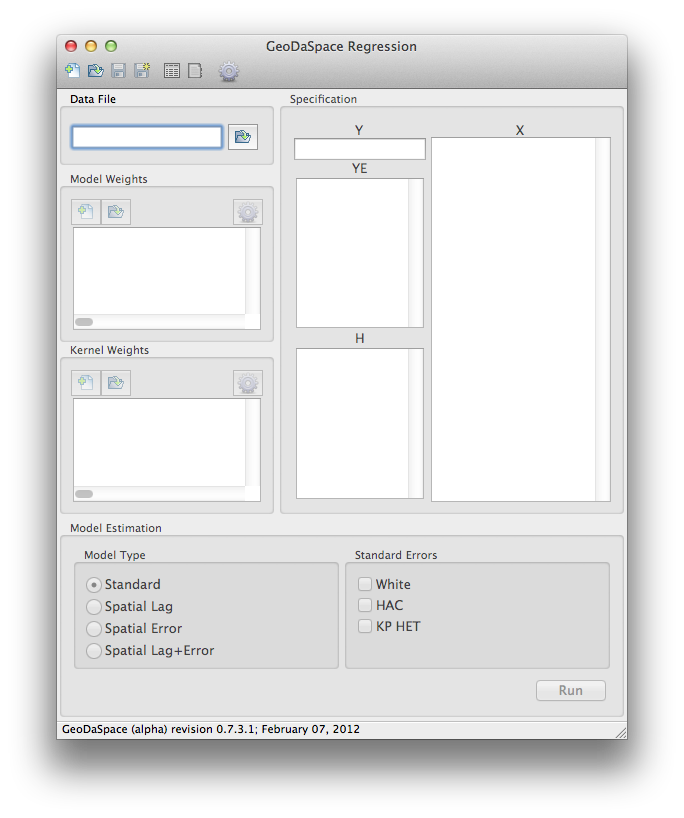
\includegraphics[width=0.8\linewidth]{GUI.png}\\
\caption{GeoDaSpace -- Main window}
\label{f:gui}
\end{center}
\end{figure}

\clearpage

The menu icons on the top of the window, from left to right, allow users to:
\begin{itemize}
\item Create a new model
\item Open an existing model
\item Save a model
\item Save a model as...
\item Open the list of variables
\item Show the results window
\item Show advanced settings (see Section \ref{s:adv})
\end{itemize}

To start the specification of a new model, users need to first open a data file. This can be done either by selecting the first menu icon `Create new model' or by selecting the open folder icon within the data file section, as shown in Figure \ref{f:opendb}.

\begin{figure}[htb]
\begin{center}
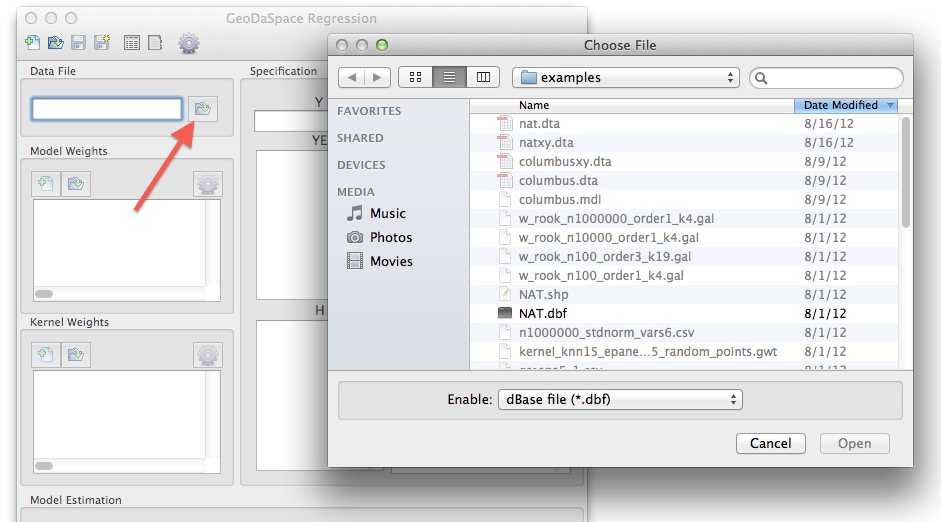
\includegraphics[width=0.9\linewidth]{opendb.png}\\
\caption{GeoDaSpace -- Open data file}
\label{f:opendb}
\end{center}
\end{figure}

Currently, GeoDaSpace can open data files in DBF, CSV and TXT formats. The examples in this document are based on the NAT.dbf file\footnote{The data used in this document are available at \url{http://geodacenter.org/downloads/data-files/ncovr.zip}. They are also part of PySAL's example data sets at \url{http://code.google.com/p/pysal/source/browse/\#svn\%2Ftrunk\%2Fpysal\%2Fexamples}}. Once the data file is open, the associated variables are listed in a separate window. This window can be retrieved any time by selecting the menu icon `Open the variable list' (second from right). To specify the model, click and drag a variable's name from the list to the respective boxes in the specification section of the main window (Figure \ref{f:spec}). The largest panel on the right, `X' (required), must contain all independent variables of the model, i.e. the explanatory or right-hand-side variables. The panel for `Y' is also required and is used for specifying the dependent or left-hand side variable. `YE'  is optional for endogenous explanatory variables; as is `H'  where the instruments for these endogenous explanatory variables can be specified.

\begin{figure}[htb]
\begin{center}
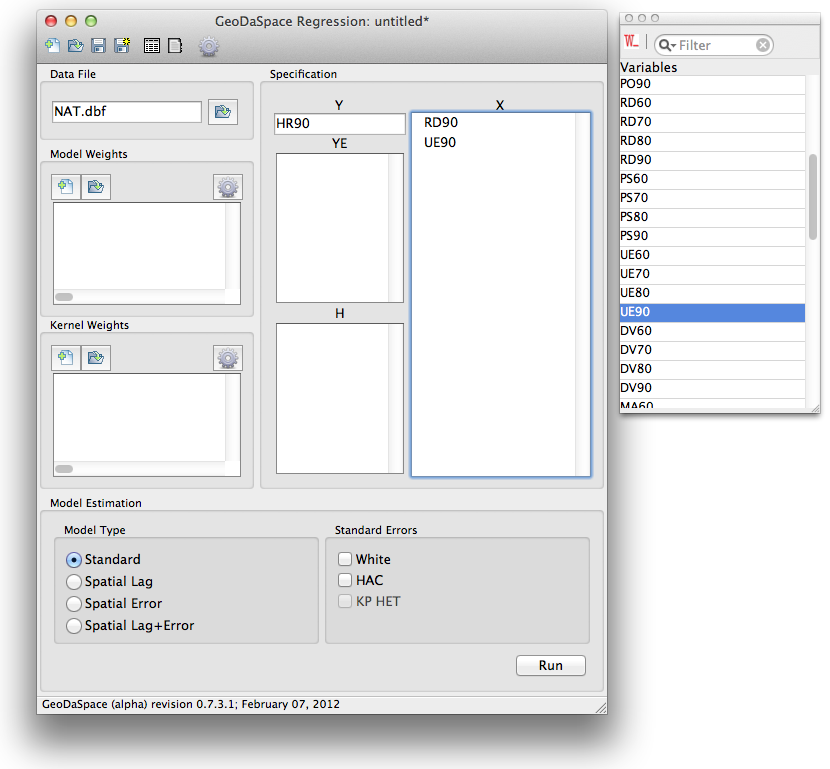
\includegraphics[width=0.9\linewidth]{spec.png}\\
\caption{GeoDaSpace -- Model specification}
\label{f:spec}
\end{center}
\end{figure}
\FloatBarrier

\subsection{Weights Creation}

The weights section allows users to create a new weights matrix or open an existing one. GeoDaSpace supports most of the common weights formats, including GAL, GWT and KWT (GeoDa weights), MAT (MatLab), TXT (Stata Text files), among others (clicking on the expandable menu of file type shows all options currently available). To create a new weights matrix the shapefile (with .shp file extension) associated with the specified data file needs to be selected  as `Input File' (Figure \ref{f:weights}). An ID variable for the weights matrix can either be selected from the data file or added by selecting the `plus' sign. 

GeoDaSpace contains two weights creation/selection panels: Model weights and kernel weights. For model weights, GeoDaSpace can create contiguity weights matrices (Queen or Rook) for any given order of contiguity based on the neighborhood structure of areas in the shapefile. Distance weights are also available (Figure \ref{f:weights}a). Euclidean and Arc distances can be used as distance metrics. The types of distance weights available are: k-nearest neighbors, binary distance bands and inverse distance. For the last two weights types it is possible to select the cut-off point and, in the case of inverse distance, the power. 

For example, to create distance weights based on the inverse of the quadratic distance, one would choose `Distance' when creating a new weights matrix, then select the `Inverse Distance' radio button and set the power to 2 (Figure \ref{f:weights}a). The cut-off point refers to the distance threshold between a given point and its neighbors.  For instance, if the metric is set to `Arc distance (miles)' and the cut-off is 100, no points farther than 100 miles from a given point will be considered as its neighbors. The default cut-off point is calculated to ensure that all spatial units have at least 1 neighbor, thus preventing the creation of units with no neighbors, i.e. islands.

\begin{figure}[htb]
\centering
\subfloat[Model weights]{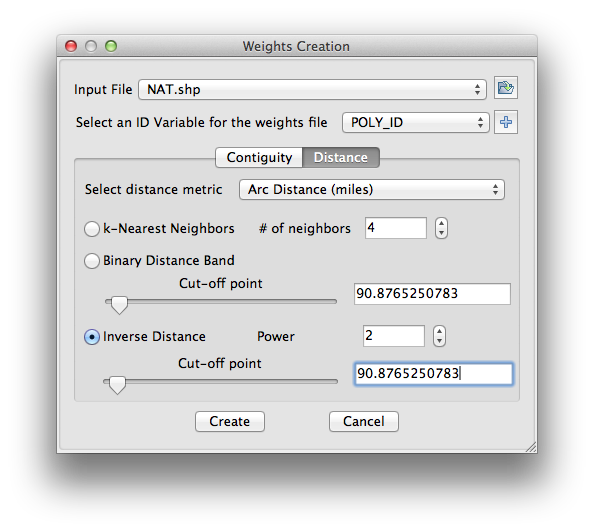
\includegraphics[width=0.5\textwidth]{distw.png}} 
\subfloat[Kernel weights]{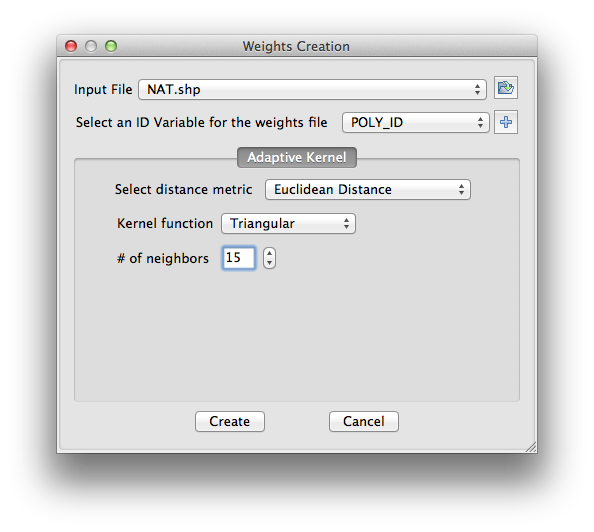
\includegraphics[width=0.5\textwidth]{kernel.png}} \\
\caption{GeoDaSpace -- Weights creation}
\label{f:weights}
\end{figure}

In addition to these standard model weights, kernel weights can be created (Figure \ref{f:weights}b). In GeoDaSpace, these are mainly used for heteroskedasticity and autocorrelation consistent (HAC) estimators \citet{Kelejian07}. Once again, Euclidean and Arc distances can be used as distance metrics. Currently, five Kernel functions are available: Uniform, Triangular, Epanechnikov, Quartic and Gaussian. It is also possible to specify the number of neighbors of each spatial unit.

The gear icon in the weights section opens a window of the properties of the selected weights matrix. In this window, it is possible to transform the weights matrix into binary, row-standardized (i.e. each row sums to 1), double-standardized (all rows sum to 1) and variance stabilized weights. The properties also include a list of the spatial units that have no neighbors, i.e. the islands, a list of the neighbors of any selected unit, the number of neighbors of each unit, i.e. the cardinalities, the unit's IDs, and a histogram of units based on the number of neighbors. As an experimental feature, it is also possible to launch an interactive viewer to visualize the neighbors of a given unit based on the specified weights matrix: The mouse can be brushed over any spatial unit of the shapefile and its neighbors are simultaneously highlighted. Note that the IDs are listed along with those of the neighbors (Figure \ref{f:viewer}).

\begin{figure}[htb]
\begin{center}
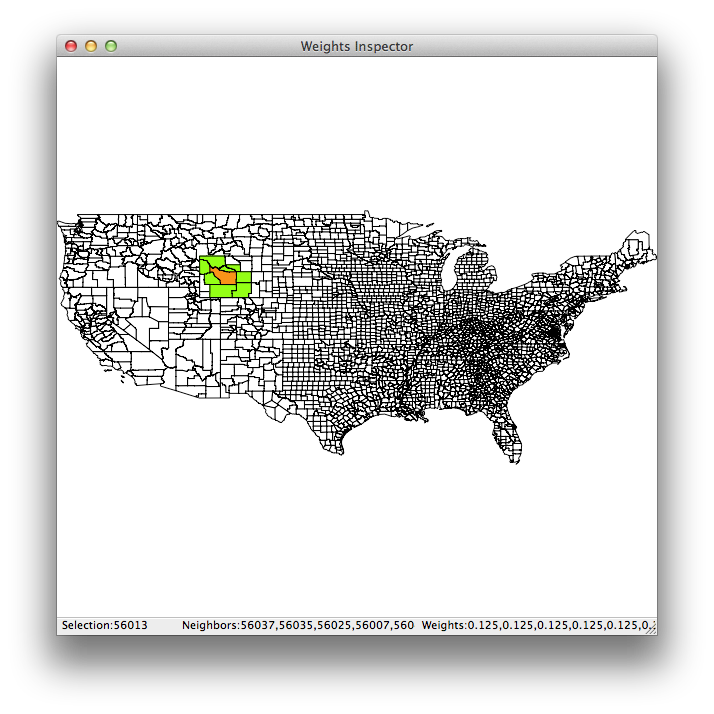
\includegraphics[width=\linewidth]{viewer.png}\\
\caption{GeoDaSpace -- Weights viewer}
\label{f:viewer}
\end{center}
\end{figure}
\FloatBarrier

\subsection{Model Estimation}
The estimation methods available in GeoDaSpace can be selected from the `Model Estimation' panel of the main window. There are four main model types: 1) standard, 2) spatial lag, 3) spatial error and 4) spatial lag and error. \\

The \textbf{standard model options} include:

\subsubsection*{Standard Options}
\begin{itemize}
      \item Ordinary least squares when no endogenous variable (YE) is specified (OLS)
     \begin{itemize}
          \item with heteroskedasticity -- White
          \item with heteroskedasticity -- HAC
      \end{itemize}
     \item Two-stage least squares  when a non-spatial endogenous variable (YE) is specified (TSLS)
      \begin{itemize}
          \item with heteroskedasticity -- White
          \item with heteroskedasticity -- HAC
         \end{itemize}
\end{itemize}

\begin{figure}[htb]
\begin{center}
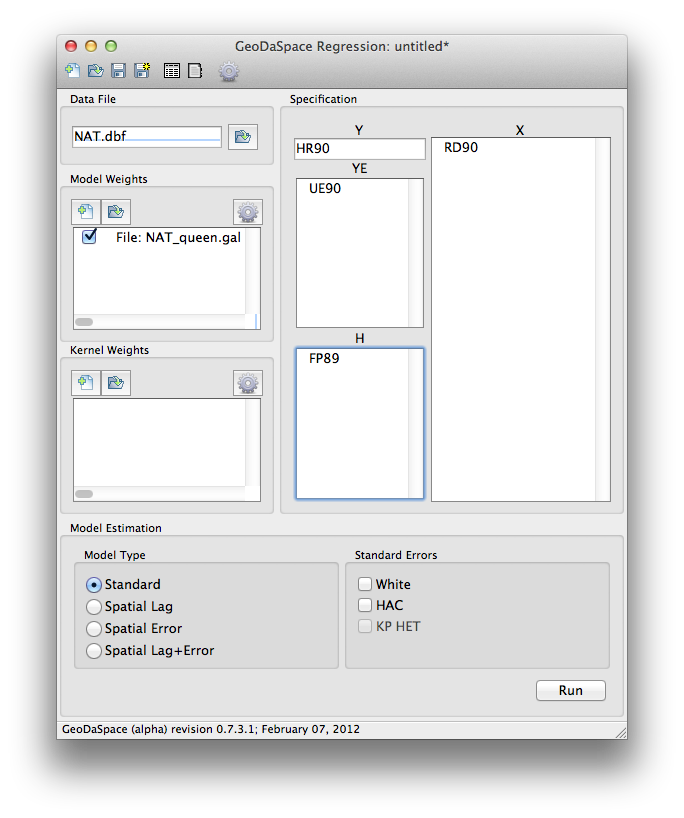
\includegraphics[width=0.7\linewidth]{tsls.png}\\
\caption{Estimation of a standard model with a non-spatial endogenous variable (YE and instrument H) using TSLS}
\label{f:tsls}
\end{center}
\end{figure}

The standard OLS and TSLS methods estimate the following model:
\begin{equation}
\mathbf{y} =  \mathbf{X}\beta + \varepsilon,
\end{equation}
where $\mathbf{y}$ is a $n \times 1$ vector containing the dependent variable `Y', $\mathbf{X}$ is a $n \times k$ matrix of observations on the explanatory variables `X', $\beta$ is a $k \times 1$ vector of coefficients, and $\varepsilon$ is a $n \times 1$ vector of random errors.

When these models are selected and run, non-spatial diagnostics and spatial diagnostics are provided if a spatial weights matrix has been selected. In case there is no variable in the 'YE' panel (implying the absence of any explanatory endogenous variable) the standard model is estimated using OLS. If instead a variable is specified in the `YE' panel, TSLS is used to estimate this model. In this case, it is also required to populate the panel `H' with the instruments for the endogenous variable (Figure \ref{f:tsls}). White and HAC corrections for heteroskedasticity (the latter requires kernel weights) are available for the standard model (both estimators). Since the `KP HET' robust estimator assumes a spatial error structure it is not available for standard model types. Section \ref{s:adv}  details advanced settings for these methods.
\FloatBarrier

For the \textbf{spatial lag model} the following options are available:

\subsubsection*{Spatial Lag Options}
\begin{itemize}
\item Spatial lag (Spatial two-stage least squares - STSLS)
     \begin{itemize}
     \item with heteroskedasticity -- White
     \item with heteroskedasticity -- HAC
     \item with non-spatial endogenous variables
     \item with non-spatial endogenous variables and heteroskedasticity -- White
     \item with non-spatial endogenous variables and heteroskedasticity -- HAC
     \end{itemize}
\end{itemize}

\begin{figure}[htb]
\begin{center}
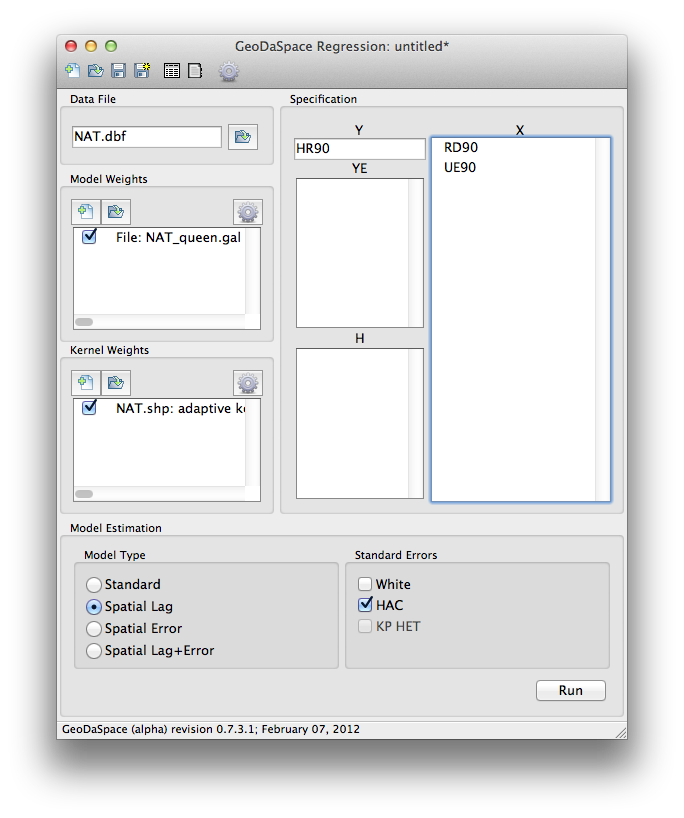
\includegraphics[width=0.7\linewidth]{haclag.png}\\
\caption{Estimation of a spatial lag model with heteroskedasticity -- HAC}
\label{f:haclag}
\end{center}
\end{figure}

The spatial lag model includes a lag of the dependent variable `Y' on the right side of the equation:
\begin{equation}
\mathbf{y} =  \rho \mathbf{W} \mathbf{y} + \mathbf{X}\beta + \varepsilon,
\end{equation}
or, alternatively:
\begin{equation}
\mathbf{y} =  (I - \rho \mathbf{W})^{-1} (\mathbf{X}\beta + \varepsilon),
\end{equation}
where $\mathbf{W}$ is the $n \times n$ spatial weights matrix and $\rho$ is the spatial autoregressive scalar parameter.

As with the standard methods described above, White and HAC corrections for heteroskedasticity are available for spatial lag models (HAC requires kernel weights). Figure \ref{f:haclag} shows an example of the estimation of a spatial lag model using the HAC to correct for heteroskedasticity. The `KP HET' robust estimator is not available for models with spatial lag models since it assumes a spatial error structure. Please see Section \ref{s:adv} for details on advanced settings for these methods.
\FloatBarrier

For the \textbf{spatial error model} the following options are available:

\subsubsection*{Spatial Error Options}
\begin{itemize}
\item Spatial error (GMM - KPD)
      \begin{itemize}
	\item with endogenous variables (GMM - KPD)
       \end{itemize}
\item Spatial error (GM - KP98/99)
      \begin{itemize}
	\item with endogenous variables (GM - KP98/99)
      \end{itemize}
\item Spatial error with heteroskedasticity (GMM - KP-Het)
      \begin{itemize}
	\item with endogenous variables and heteroskedasticity  (GMM - KP-Het)
      \end{itemize}
\end{itemize}

\begin{figure}[htb]
\begin{center}
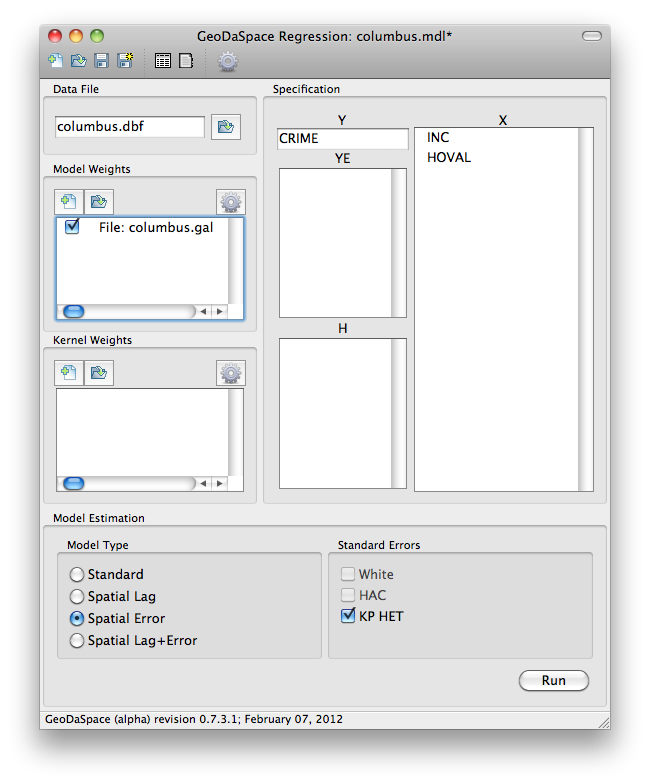
\includegraphics[width=0.7\linewidth]{GS_het.png}\\
\caption{Estimation of spatial error models with heteroskedasticity}
\label{f:GS_het}
\end{center}
\end{figure}

The spatial error model estimates a spatial autoregressive parameter in the errors ($\lambda$):
\begin{equation}
\mathbf{y} =  \mathbf{X}\beta + \mathbf{u},
\end{equation}
\begin{equation}
\mathbf{u} =  \lambda \mathbf{W} \mathbf{u} + \varepsilon,
\end{equation}
or, alternatively:
\begin{equation}
\mathbf{y} =  \mathbf{X}\beta + (I - \lambda \mathbf{W})^{-1} \varepsilon.
\end{equation}

GeoDaSpace provides two different estimators for spatial error models without heteroskedasticity. The default is the GMM estimator proposed by \citet{Drukker10}, which we refer to as `KPD'. The second option is the GM estimator proposed by \citet{Kelejian98,Kelejian99}, here referred as `KP98/99'. The choice of the estimator to be used can be changed in the Advanced Settings Panel (Section \ref{s:adv}). Given the spatial structure of the error term, it is not possible to use White or HAC corrections for heteroskedasticity. Instead, GeoDaSpace estimates the method proposed by \citet{Arraiz10}, which is robust to heteroskedasticity. To estimate this method, both the `Spatial Error' model and `KP HET' standard errors need to be selected (Figure \ref{f:GS_het}). Please see Section \ref{s:adv} for details on advanced settings for these methods.
\FloatBarrier

For the \textbf{spatial lag and error model} the following options are available:

\subsubsection*{Spatial Lag and Error Options}
\begin{itemize}
\item Spatial lag and error (KPD)
	\begin{itemize}
	\item with additional endogenous variables (KPD)
	\end{itemize}
\item Spatial lag and error (KP98/99)
	\begin{itemize}
	\item with additional endogenous variables (KP98/99)
	\end{itemize}
\item Spatial lag and error with heteroskedasticity (GMM - KP-Het)
	\begin{itemize}
	\item with additional endogenous variables and heteroskedasticity (GMM - KP-Het)
	\end{itemize}
\end{itemize}

The spatial lag and error model estimates spatial autoregressive parameters both in the errors ($\lambda$) and for the spatial lag of the dependent variable ($\rho$):
\begin{equation}
\mathbf{y} = \rho \mathbf{W} \mathbf{y} + \mathbf{X}\beta + \mathbf{u},
\end{equation}
\begin{equation}
\mathbf{u} =  \lambda \mathbf{W} \mathbf{u} + \varepsilon,
\end{equation}
or, alternatively:
\begin{equation}
\mathbf{y} =  (I - \rho \mathbf{W})^{-1} \mathbf{X}\beta + (I - \rho \mathbf{W})^{-1}(I - \lambda \mathbf{W})^{-1} \varepsilon.
\end{equation}


\begin{figure}[htb]
\centering
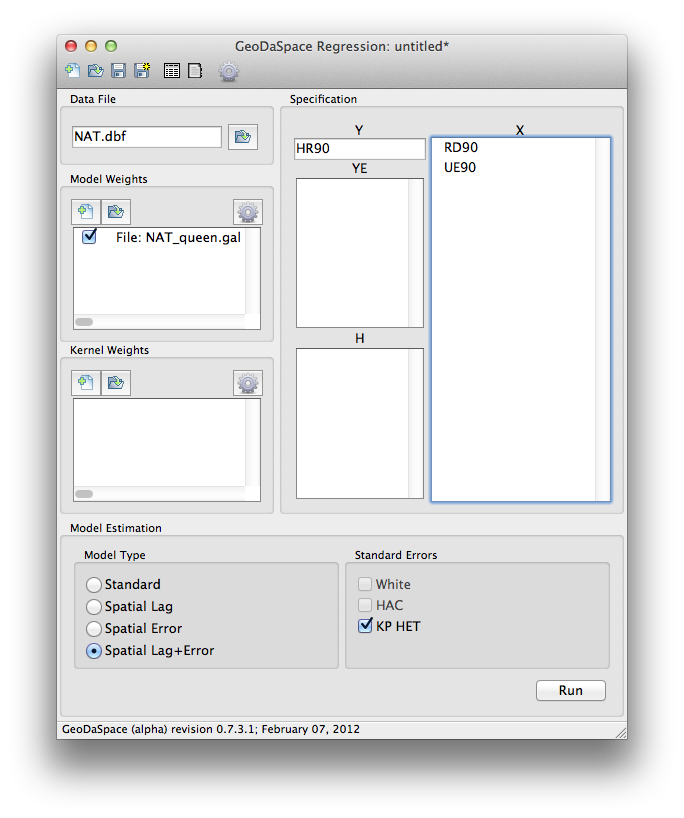
\includegraphics[width=0.7\textwidth]{GS_het_combo.png}
\caption{Estimation of spatial lag and error model with heteroskedasticity}
\label{f:GS_het_combo}
\end{figure}

All estimation methods for the spatial error model are also available for the spatial lag and error model. Here again, the default is the `KPD' estimator but the `KP98/99' estimator can be selected from the Advanced Settings Panel (Section \ref{s:adv}). In the presence of heteroskedasticity, it is possible to estimate the method proposed by \citet{Arraiz10} by selecting both the `Spatial Lag+Error' model and `KP HET' standard errors. Figure \ref{f:GS_het_combo} shows how to estimate a spatial error model with spatial lag and heteroskedasticity in GeoDaSpace.
\FloatBarrier


\subsection{Advanced Settings}
\label{s:adv}


The advanced settings window offers several options to customize the methods implemented in GeoDaSpace. To access this window, select the gear icon on the top menu. (Figure \ref{f:gui_adv}).
 
\begin{figure}[htb]
\centering
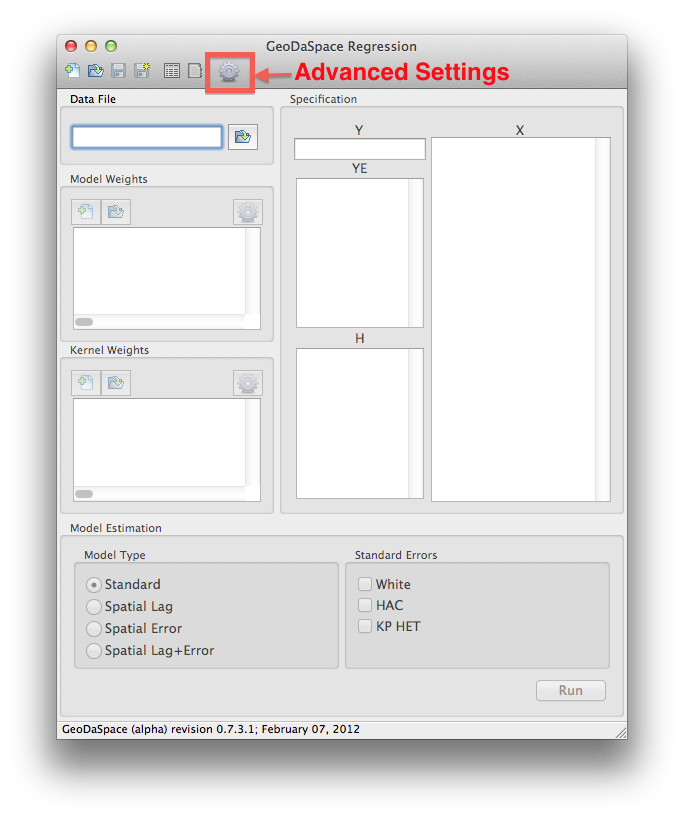
\includegraphics[width=0.9\textwidth]{GUI_adv.png}
\caption{Advanced settings panel}
\label{f:gui_adv}
\end{figure}
\FloatBarrier

\begin{figure}[htb]
\centering
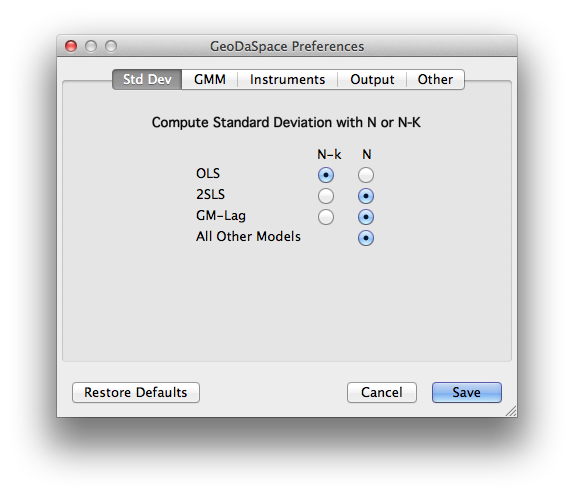
\includegraphics[width=0.7\textwidth]{adv_std.png}
\caption{Advanced settings panel -- Standard Deviations}
\label{f:adv_std}
\end{figure}

The first tab of the advanced settings panel is related to the way GeoDaSpace computes the standard deviation for all methods (Figure \ref{f:adv_std}). The formula for the normalization used in the calculation of the standard deviations can be selected for the OLS, TSLS, GM-lag and all other models. By default, the denominator is only set to $(N-k)$ in the OLS case. For all others, the default is $N$. If $N$ is very large, the difference between both choices will decrease. However, the results for small samples can vary depending on which of these options is selected.
\FloatBarrier

\begin{figure}[htb]
\centering
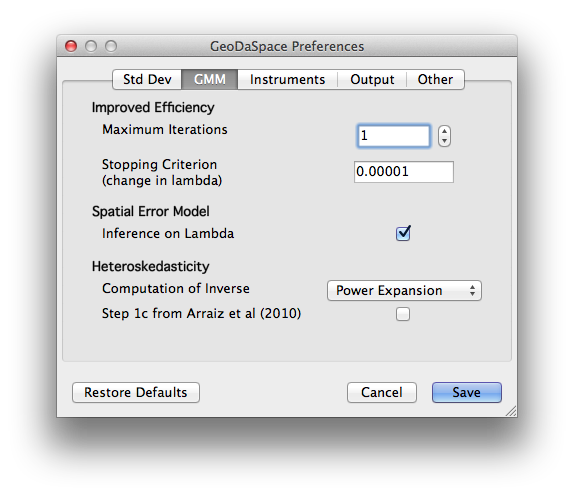
\includegraphics[width=0.7\textwidth]{adv_gmm.png}
\caption{Advanced settings panel -- GMM}
\label{f:adv_gmm}
\end{figure}

The second tab is related to the estimation of the GMM methods in GeoDaSpace (Figure \ref{f:adv_gmm}). Estimators such as the KPD spatial error method \citep{Drukker10} and spatial error with heteroskedasticity KP-HET \citep{Arraiz10} allow for several iterations to improve efficiency (see \citet{Anselin11} for details). The maximum number of iterations can be selected in this tab, as well as the convergence criterion. When any of these two criteria is achieved, the iteration process is finalized. In other words, when the difference between two subsequent estimations of $\lambda$ is less or equal than the value assigned in the convergence criterion box or when the maximum number of iterations is reached, no more iterations are performed.

The second item in this tab refers to the inference on $\lambda$ in spatial error or spatial lag and error models. When there is no heteroskedasticity, this option defines if the estimation method selected is the KP98/99 or the KPD. The default, when the box is checked, provides the inference on $\lambda$ by estimating the KPD model. As originally proposed by \citet{Kelejian98,Kelejian99}, the estimation of the KP98/99 does not provide this inference. The KP98/99 is the method used when the box is unchecked.

The third and last item in the GMM tab is related to the estimation of spatial error models with heteroskedasticity. Here one can select the method for the computation of the inverse of the operations involving the $\mathbf{W}$ matrix. By default, a power expansion is performed in these cases, so that the computational time is decreased. If instead the true inverse is desired, this option is available from the drop-down list. 

In addition, one can also opt to include step 1c in the estimation of the spatial error model with heteroskedasticity, as proposed by \citet{Arraiz10}. Step 1c updates the initial consistent estimation of lambda using a weighted nonlinear least squares solution to the moments equations. This results in a consistent and efficient intermediate estimation of $\lambda$. Note, however, that a consistent estimation at this stage is already sufficient to obtain a consistent estimation of all parameters in the model. For this reason, the default in GeoDaSpace is set to skip this step to save computational time.
\FloatBarrier

\begin{figure}[htb]
\centering
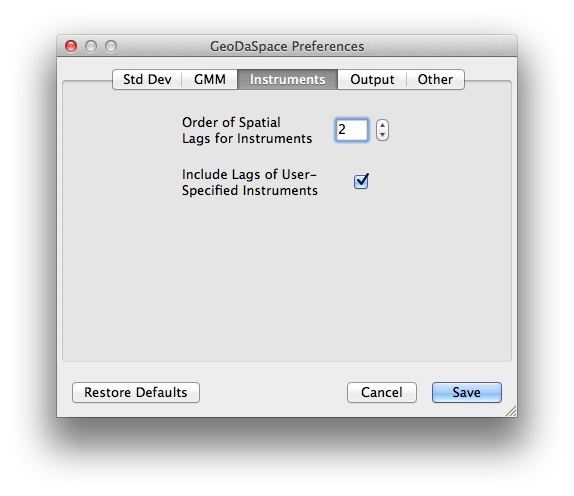
\includegraphics[width=0.7\textwidth]{adv_inst.png}
\caption{Advanced settings panel -- Instruments}
\label{f:adv_inst}
\end{figure}

The third tab is the Instruments tab (Figure \ref{f:adv_inst}). In this tab it is possible to change the way GeoDaSpace deals with instruments for spatial lag as well as spatial lag and error models. The first item refers to the order of the spatial lags of the exogenous variables that are used as instruments of the spatial lag of the dependent variable. The default is to only use the first order lags of these variables, i.e. $\mathbf{WX}$, as instruments for $\mathbf{Wy}$. If instead we change the order of the spatial lags for instruments to 2, $\mathbf{WX}+ \mathbf{W^2X}$ will be used as instruments. 

The second checkbox, checked by default, determines the inclusion of the spatial lag of the user-specified instruments in addition to the lag of the exogenous variables (this applies when instruments are specified in the `H' panel of the main GUI). The instruments in this case are $\mathbf{WX} + \mathbf{WH}$.
\FloatBarrier

\begin{figure}[htb]
\centering
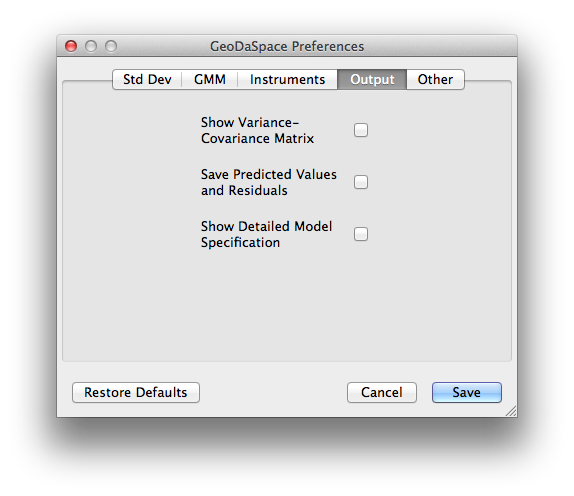
\includegraphics[width=0.7\textwidth]{adv_out.png}
\caption{Advanced settings panel -- Output}
\label{f:adv_out}
\end{figure}
\FloatBarrier

The fourth tab is related to the output that GeoDaSpace prints in the results window (Figure \ref{f:adv_out}).  The first checkbox controls the printing of the $k \times k$ variance-covariance matrix of the estimated parameters. When the box is checked (default is off), the variance-covariance matrix will be displayed below the main estimation results.

The second item allows us to save the predicted values of the dependent variable and residuals to a data file. If this option is checked, GeoDaSpace creates a CSV files containing this information. Before the estimation is performed, a pop-up window allows us to choose the folder and filename.

The last item in the Output box is ``Show Detailed Model Specification.'' This option is currently under development and not yet available. Selecting it will not affect the output in the current version.

The last tab contains other type of options. The first item refers to the calculation of regression diagnostics. By default, non-spatial diagnostics are calculated when running an OLS model. These diagnostics include the Jarque-Bera normality test, heteroskedasticity and multicollinearity diagnostics. The next item is related to the calculation of the Moran's I test for spatial dependence. When a spatial weights matrix is selected with a standard model, the results for Lagrange Multiplier (LM) tests are calculated and shown in the results window. When the box for the Moran's I is checked in the advanced settings panel, the Moran's I test results are also included. By default this option is not selected since the calculation of Moran's I increases the computation time, especially for large samples.

\begin{figure}[htb]
\centering
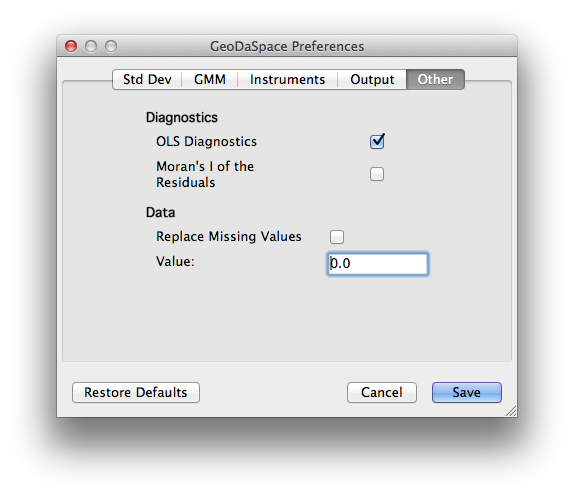
\includegraphics[width=0.7\textwidth]{adv_other.png}
\caption{Advanced settings panel -- Other}
\label{f:adv_other}
\end{figure}

The second group of items in this tab refers to data manipulation. Currently GeoDaSpace cannot deal with missing values in the data. When these exist, this option allows users to replace all missing values with a given value (zero by default).

It is possible to save all options in the advanced settings panel. By selecting the `Save' button, these chosen options will be saved for future sessions of GeoDaSpace, not only for the model that is currently estimated. It is also possible to restore the default values at any time by selecting the 'Restore Defaults' option in this tab and then saving these changes.

%\newpage

\section{Comparison of Results: GeoDaSpace, Stata and R}
\label{s:comparisons}

\subsection{Introduction}
As Table \ref{t:methods} showed, the methods implemented in GeoDaSpace are also available in Stata or R. Some of the results of different types of spatial error models vary across these three programs. The purpose of this section is to explain these divergent results. Further, we demonstrate how to set the preferences in GeoDaSpace or customize the underlying PySAL code in order to obtain consistent results across programs.\footnote{As mentioned, more information on PySAL can be found at \url{http://pysal.org/}} \citep{Rey07}.

For this comparison we use two different versions of the R package \emph{sphet}. The first one, henceforth \emph{sphet1}, is the released version of \emph{sphet} (v. 1.1-12, published on CRAN on 2012-04-13). In addition to this version of \emph{sphet}, we also use the alpha version from R-Forge, revision 56, published on 2012-07-22. This newer version of the code, which contains many additional methods and enhancements to \emph{sphet1}, will be referred to as \emph{sphet2}\footnote{Given that it is an alpha version, the code is subject to change.}.


The following spatial error models are discussed in this section:

\begin{itemize}
\item Spatial error models (KPD) with 
	\begin{itemize}
	\item exogenous variables and no heteroskedasticity
	\item endogenous variables and no heteroskedasticity
	\item spatial lag and no heteroskedasticity
	\item exogenous variables and heteroskedasticity
	\item endogenous variables and heteroskedasticity
	\item spatial lag and heteroskedasticity
	\end{itemize}
\end{itemize}

\subsection{Spatial Error Models without Heteroskedasticity}

The default GMM estimator for the spatial error model without heteroskedasticity in GeoDaSpace is the KPD \citep{Drukker10}. Given the particular specification of this model when all variables are exogenous (see \citet{Anselin11}), the results from GeoDaSpace do not match those from Stata. This discrepancy is due to the fact that, for the case of a spatial error model with exogenous variables only, Stata ignores the exogeneity and uses two-stage least squares rather than OLS.

To demonstrate this point, PySAL's base classes are used to match Stata's results because they include more customization options than are available in GeoDaSpace. Since Stata's results are based on 2SLS rather than OLS estimation, one has to specify $\mathbf{X}$ as both the endogenous variables and the instruments in PySAL in order to match Stata's results. PySAL requires at least one exogenous variable - hence, a constant needs to be included. Listing \ref{lt:hom_stata} shows the command to match PySAL's and Stata's results for the spatial error model\footnote{A description of the estimation of spatial error models without heteroskedasticity using PySAL can be found at \url{http://pysal.geodacenter.org/dev/library/spreg/error_sp_hom.html}}. 

In addition to the different treatment of the exogenous variables in Stata, the A1 matrix used to estimate the model is also different in the two programs. In PySAL's code and GeoDaSpace's, the option for the use of the matrix is based on \citet{Arraiz10} instead of \citet{Drukker10} and \citet{Drukker11}. The details of this choice are outlined in \citet{Anselin11}.  

Table \ref{t:res_hom} compares the results from GeoDaSpace, Stata and R. The KPD method is not available in the currently released version of \emph{sphet1} (v. 1.1-12). However, the results presented here can be obtained using \emph{sphet2}, the alpha version from R-Forge\footnote{For this document we use revision 56, published on 2012-07-22.}. As Table \ref{t:res_hom} shows, the results from GeoDaSpace differ from those of \emph{sphet2}. 

\begin{table}[htpb]
\caption{Comparison of the results of spatial error models with exogenous variables and no heteroskedasticity}
\label{t:res_hom}
\centering
\begin{small}
\begin{tabular}{l|cccc} \hline
\textbf{Variable}&\textbf{GeoDaSpace}&\textbf{sphet2}&\textbf{Stata}&\textbf{PySAL$^1$}\\ \hline
CONSTANT&8.0259&6.6762&6.9884&6.9884\\
&(0.3601)&(0.3498)&(0.3605)&(0.3605)\\
RD90&4.3228&3.9450&3.9945&3.9945\\
&(0.1596)&(0.1553)&(0.1612)&(0.1612)\\
UE90&-0.2753&-0.0770&-0.1240&-0.1240\\
&(0.0479)&(0.0471)&(0.0490)&(0.0490)\\
lambda&0.4572&0.4149&0.4124&0.4124\\
&(0.0189)&(0.0194)&(0.0194)&(0.0194)\\
\hline
\multicolumn{5}{l}{\scriptsize{$^1$PySAL using the code to match Stata as in Listing \ref{lt:hom_stata}.}} \\
\end{tabular}
\end{small}
\end{table}




\begin{code}
\begin{lstlisting}[label=lt:hom_stata,caption=Using PySAL to match the results of spatial error models from Stata,language=Python]

import pysal
import numpy as np

w = pysal.open('NAT_queen.gal').read()
w.transform = 'r'
db = pysal.open('NAT.dbf')
hr90 = np.array([db.by_col('HR90')]).T
rd90 = np.array([db.by_col('RD90')]).T
ue90 = np.array([db.by_col('UE90')]).T
x = np.hstack((rd90,ue90))

ones = np.ones(crime.shape)
model = pysal.spreg.BaseGM_Endog_Error_Hom(hr90, ones,
        yend=x, q=x, w=w, A1='hom_sc')

print model.betas
print map(np.sqrt, model.vm.diagonal())

\end{lstlisting}
\end{code}

When endogenous variables, including a spatial lag, are specified, Stata uses a 2SLS estimator instead of OLS. Nonetheless, the results from GeoDaSpace still diverge from Stata's and R's, as shown in Table \ref{t:res_hom_endog}. The diffence is due to the choice of the A1 matrix used in the estimations and, for the spatial lag, the number of lags of the exogenous variables used as instruments.  

\begin{table}[htpb]
\caption{Comparison of the results of spatial error models with endogenous variables or spatial lag}
\label{t:res_hom_endog}
\centering
\begin{small}
\begin{tabular}{l|cccc} \hline
\multicolumn{5}{c}{\textbf{Spatial error with UE90 as endogenous variable}} \\ \hline
\textbf{Variable}&\textbf{GeoDaSpace}&\textbf{sphet2}&\textbf{Stata}&\textbf{PySAL$^1$}\\ \hline
CONSTANT&21.0288&19.7052&21.0606&21.0606\\
&(1.5362)&(1.4194)&(1.5385)&(1.5385)\\
RD90&8.2376&8.0369&8.2420&8.2420\\
&(0.4881)&(0.4634)&(0.4888)&(0.4888)\\
UE90$^2$&-2.2392&-2.0396&-2.2438&-2.2438\\
&(0.2286)&(0.2111)&(0.2290)&(0.2290)\\
lambda&0.4934&0.4856&0.4944&0.4944\\
&(0.0216)&(0.0220)&(0.0217)&(0.0217)\\
\hline
\multicolumn{5}{c}{\textbf{Spatial error with spatial lag}} \\ \hline
\textbf{Variable}&\textbf{GeoDaSpace$^3$}&\textbf{sphet2}&\textbf{Stata}&\textbf{PySAL$^1$}\\ \hline
CONSTANT&6.9406&6.9362&6.9362&6.9362\\
&(0.5327)&(0.5120)&(0.5120)&(0.5120)\\
RD90&4.0074&4.0061&4.0061&4.0061\\
&(0.1758)&(0.1764)&(0.1764)&(0.1764)\\
UE90&-0.0957&-0.0978&-0.0978&-0.0978\\
&(0.0490)&(0.0481)&(0.0481)&(0.0481)\\
W\_HR90&-0.0220&-0.0190&-0.0190&-0.0190\\
&(0.0543)&(0.0513)&(0.0513)&(0.0513)\\
lambda&0.5098&0.4364&0.4364&0.4364\\
&(0.0376)&(0.0421)&(0.0421)&(0.0421)\\
\hline
\multicolumn{5}{l}{\scriptsize{$^1$PySAL using the code to match Stata as in Listing \ref{lt:hom_end_stata}.}} \\
\multicolumn{5}{l}{\scriptsize{$^2$UE90 instrumented by FP89 and all other exogenous variables.}} \\
\multicolumn{5}{l}{\scriptsize{$^3$GeoDaSpace using 2 spatial lags for the instruments.}} \\
\multicolumn{5}{l}{\scriptsize{\hl{Note: I'm still not convinced I'm doing the endog model in R right.}}} \\
\multicolumn{5}{l}{\scriptsize{\hl{I'll have to check with Gianfranco. He says his results match Stata's.}}} \\
\end{tabular}
\end{small}
\end{table}

PySAL can again be used to match the results of Stata. Listing \ref{lt:hom_end_stata} illustrates that when the option `hom\_sc' is selected for the argument A1 the default A1=`het' is overridden. Hence, the matrix A1 as defined in \citet{Arraiz10} is replaced by A1 as defined in \citet{Drukker10} and \citet{Drukker11}. For the case of a spatial lag, it is also important to change the number of spatial lags of the exogenous variables that will be used as instruments of the spatial lag of the dependent variable. The default used in GeoDaSpace is `1'. The value must be changed to `2' in order to match Stata's results. The code shown in Listing \ref{lt:hom_end_stata} is a continuation of Listing \ref{lt:hom_stata}.

\begin{code}
\begin{lstlisting}[label=lt:hom_end_stata,caption=Using PySAL to match the results of spatial error models with endogenous variables or spatial lag from Stata,language=Python]

#Spatial error model with spatial lag:
model = pysal.spreg.GM_Combo_Hom(hr90, x, w=w, 
        A1='hom_sc', w_lags=2)
print model.summary

#Adding instrument 'FP89':
fp89 = np.array([db.by_col('FP89')]).T

#Spatial error model with UE90 as endogenous variable:
model = pysal.spreg.GM_Endog_Error_Hom(hr90, rd90,
        yend=ue90, q=fp89, w=w, A1='hom_sc')
print model.summary

\end{lstlisting}
\end{code}

\subsection{Spatial Error Models with Heteroskedasticity}

As in the case with no heteroskedasticity, Stata's code for the estimation of the spatial error model with exogenous variables cannot be matched with the results of GeoDaSpace. Table \ref{t:res_het} compares GeoDaSpace's results with those of Stata and R's \emph{sphet} package.\footnote{As stated before, we refer to the released version 1.1-12 of \emph{sphet} as \emph{sphet1} and the updated alpha version of \emph{sphet} available from R-Forge (revision 56 published on 2012-07-22) as \emph{sphet2}.} In contrast to \emph{sphet2}, \emph{sphet1} does not include the option to skip one step in the estimation of the method (step1c), which is done by default in GeoDaSpace, Stata and \emph{sphet2}. Please check Section \ref{s:step1c} for more details on this.

\begin{table}[htpb]
\caption{Comparison of the results of spatial error models with exogenous variables and heteroskedasticity}
\label{t:res_het}
\centering
\begin{small}
\begin{tabular}{l|ccccc} \hline
\textbf{Variable}&\textbf{GeoDaSpace}&\textbf{sphet1}&\textbf{sphet2}&\textbf{Stata}&\textbf{PySAL$^1$}\\ \hline
CONSTANT&6.6586&6.5782&6.6586&6.9777&6.9777\\
&(0.4749)&(0.4594)&(0.4745)&(0.4622)&(0.4622)\\
RD90&3.9417&3.9275&3.9417&3.9911&3.9911\\
&(0.2602)&(0.2316)&(0.2599)&(0.2326)&(0.2325)\\
UE90&-0.0745&-0.0630&-0.0745&-0.1225&-0.1225\\
&(0.0611)&(0.0589)&(0.0611)&(0.0592)&(0.0592)\\
lambda&0.4753&0.4756&0.4740&0.4721&0.4721\\
&(0.0235)&(0.0237)&(0.0237)&(0.0236)&(0.0236)\\
\hline
\multicolumn{6}{l}{\scriptsize{$^1$PySAL using the code to match Stata as in Listing \ref{lt:het_stata}.}} \\
\end{tabular}
\end{small}
\end{table}

In PySAL, it is possible to mimic Stata's code to estimate a model that yields the same results\footnote{A description of the estimation of spatial error models with heteroskedasticity using PySAL can be found at \url{http://pysal.geodacenter.org/dev/library/spreg/error_sp_het.html}}. The code is shown in Listing \ref{lt:het_stata}.

\begin{code}
\begin{lstlisting}[label=lt:het_stata,caption=Using PySAL to match the results of spatial error models with heteroskedasticity from Stata,language=Python]

import pysal
import numpy as np

w = pysal.open('NAT_queen.gal').read()
w.transform = 'r'
db = pysal.open('NAT.dbf')
hr90 = np.array([db.by_col('HR90')]).T
rd90 = np.array([db.by_col('RD90')]).T
ue90 = np.array([db.by_col('UE90')]).T
x = np.hstack((rd90,ue90))

model = pysal.spreg.BaseGM_Endog_Error_Het(hr90, ones,
        yend=x, q=x, w=w)

print model.summary

\end{lstlisting}
\end{code}

When the spatial error model with heteroskedasticity contains a spatial lag, the default specification in GeoDaSpace does match the results from Stata. This is due to the order of the spatial lags of the exogenous variables used as instruments of the spatial lag of the dependent variable. The default in GeoDaSpace is a single lag. In Stata, however, the exogenous variables are lagged twice. This option cannot be changed in Stata. In GeoDaSpace, the number of lags can be changed in the Preferences Panel (see Section \ref{s:adv}). When `2' is selected as the order of spatial lags for instruments, the results from GeoDaSpace match Stata's, as shown in Table \ref{t:res_het_combo}. 
\begin{table}[htpb]
\caption{Comparison of the results of spatial error models with spatial lag and heteroskedasticity}
\label{t:res_het_combo}
\centering
\begin{small}
\begin{tabular}{l|ccccc} \hline
\textbf{Variable}&\textbf{GeoDaSpace$^1$}&\textbf{sphet1}&\textbf{sphet2}&\textbf{Stata}&\textbf{PySAL$^2$}\\ \hline
CONSTANT&6.9406&7.0196&6.9406&6.9406&6.9406\\
&(0.8600)&(0.8251)&(0.8600)&(0.8600)&(0.8600)\\
RD90&4.0074&4.0057&4.0074&4.0074&4.0074\\
&(0.3261)&(0.3212)&(0.3261)&(0.3261)&(0.3261)\\
UE90&-0.0957&-0.0643&-0.0957&-0.0957&-0.0957\\
&(0.0664)&(0.0640)&(0.0664)&(0.0664)&(0.0664)\\
W\_HR90&-0.0220&-0.0702&-0.0220&-0.0220&-0.0220\\
&(0.0876)&(0.0839)&(0.0876)&(0.0876)&(0.0876)\\
lambda&0.5584&0.6399&0.5584&0.5584&0.5584\\
&(0.0507)&(0.0460)&(0.0507)&(0.0507)&(0.0507)\\
\hline
\multicolumn{6}{l}{\scriptsize{$^1$GeoDaSpace using 2 spatial lags for the instruments.}} \\
\multicolumn{6}{l}{\scriptsize{$^2$PySAL using the code to match Stata as in Listing \ref{lt:het_endog_stata}.}} \\
\end{tabular}
\end{small}
\end{table}

If the spatial error model with heteroskedasticity contains other type of endogenous variables, but not a spatial lag, the results from GeoDaSpace match those from Stata without the need of any change (Table \ref{t:res_het_endog}).

\begin{table}[htpb]
\caption{Comparison of the results of spatial error models with endogenous variable (UE90) and heteroskedasticity}
\label{t:res_het_endog}
\centering
\begin{small}
\begin{tabular}{l|cccc} \hline
\textbf{Variable}&\textbf{GeoDaSpace}&\textbf{sphet2$^1$}&\textbf{Stata}&\textbf{PySAL$^2$}\\ \hline
CONSTANT&21.0288&19.6812&21.0288&21.0288\\
&(2.5629)&(2.2653)&(2.5629)&(2.5629)\\
RD90&8.2376&8.0401&8.2376&8.2376\\
&(0.7817)&(0.7161)&(0.7817)&(0.7817)\\
UE90$^3$&-2.2392&-2.0361&-2.2392&-2.2392\\
&(0.3902)&(0.3449)&(0.3902)&(0.3902)\\
lambda&0.4667&0.4614&0.4667&0.4667\\
&(0.0298)&(0.0295)&(0.0298)&(0.0298)\\
\hline
\multicolumn{5}{l}{\scriptsize{$^1$sphet1 does not allow for endogenous variables.}} \\
\multicolumn{5}{l}{\scriptsize{$^2$PySAL using the code to match Stata as in Listing \ref{lt:het_endog_stata}.}} \\
\multicolumn{5}{l}{\scriptsize{$^3$UE90 instrumented by FP89 and exogenous variables.}} \\
\multicolumn{5}{l}{\scriptsize{\hl{Note: I'm still not convinced I'm doing the endog model in R right.}}} \\
\multicolumn{5}{l}{\scriptsize{\hl{I'll have to check with Gianfranco. He says his results match Stata's.}}} \\
\end{tabular}
\end{small}
\end{table}


In PySAL, these models could be estimated using the code shown in Listing \ref{lt:het_endog_stata}. This code is a continuation of Listing \ref{lt:het_stata}.

\begin{code}
\begin{lstlisting}[label=lt:het_endog_stata,caption=Using PySAL to match the results of spatial error models with heteroskedasticity and endogenous variables or spatial lag from Stata,language=Python]

#Spatial error model with spatial lag and
#    heteroskedasticity:
model = pysal.spreg.GM_Combo_Het(hr90, x,
        w=w, w_lags=2)
print model.summary

#Adding instrument 'FP89':
fp89 = np.array([db.by_col('FP89')]).T

#Spatial error model with UE90 as endogenous variable
#    and heteroskedasticity:
model = pysal.spreg.GM_Endog_Error_Het(hr90, rd90,
        yend=ue90, q=fp89, w=w)
print model.summary

\end{lstlisting}
\end{code}
\FloatBarrier


\subsubsection{Initial Efficient Estimation of Lambda (Step1c)}
\label{s:step1c}
In addition to the number of lags of the exogenous variables used as instruments, both GeoDaSpace and PySAL also offer the possibility to add the Step 1c in the estimation of the model as proposed by \citet{Arraiz10}. Step 1c updates the initial consistent estimation of lambda using a weighted nonlinear least squares solution to the moments equations. This results in a consistent and efficient intermediate estimation of lambda. Note, however, that a consistent estimation at this stage is already sufficient to obtain a consistent estimation of all parameters in the model. The option to run Step 1c can be found in the preferences panel in GeoDaSpace, as shown in Section \ref{s:adv}. In PySAL, this option can be selected by adding `step1c=True' to the arguments of the model (Listing \ref{lt:het_step1c}).

\begin{code}
\begin{lstlisting}[label=lt:het_step1c,caption=Using PySAL to match the results of spatial error models with heteroskedasticity and endogenous variables or spatial lag from Stata,language=Python]

#Spatial error model with heteroskedasticity
#    (running Step1c):
model = pysal.spreg.GM_Error_Het(hr90, x,
        w=w, step1c=True)
print model.summary

#Spatial error model with spatial lag and
#    heteroskedasticity (running Step1c):
model = pysal.spreg.GM_Combo_Het(hr90, x,
        w=w, step1c=True)
print model.summary

#Spatial error model with HOVAL as endogenous variable
#    and heteroskedasticity (running Step1c):
model = pysal.spreg.GM_Endog_Error_Het(hr90, rd90,
        yend=ue90, q=fp89, w=w, step1c=True)
print model.summary

\end{lstlisting}
\end{code}


\newpage
\bibliography{bib}
\bibliographystyle{apalike}
\end{document}




